\documentclass{article}
\usepackage{tikz}

\begin{document}

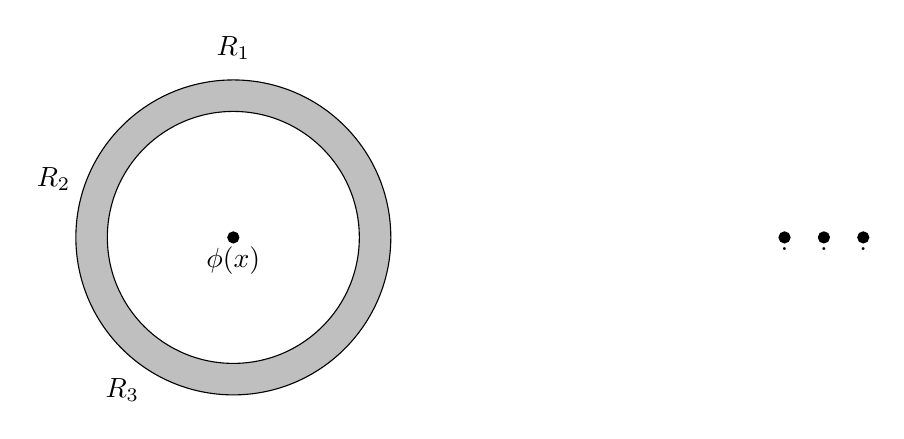
\begin{tikzpicture}[scale=2]
    % Draw the outer circle
    \draw[fill=gray!50] (0,0) circle (1);
    
    % Draw the inner circle
    \draw[fill=white] (0,0) circle (0.8);
    
    % Label the regions
    \node at (90:1.2) {$R_1$};
    \node at (162:1.2) {$R_2$};
    \node at (234:1.2) {$R_3$};
    
    % Add the dot and label
    \filldraw (0,0) circle (1pt) node[anchor=north] {$\phi(x)$};
    
    % Add the dots for the legend
    \filldraw (3.5,0) circle (1pt) node[anchor=north] {.};
    \filldraw (3.75,0) circle (1pt) node[anchor=north] {.};
    \filldraw (4,0) circle (1pt) node[anchor=north] {.};
\end{tikzpicture}

\end{document}